\begin{figure}[h] 
\centering 
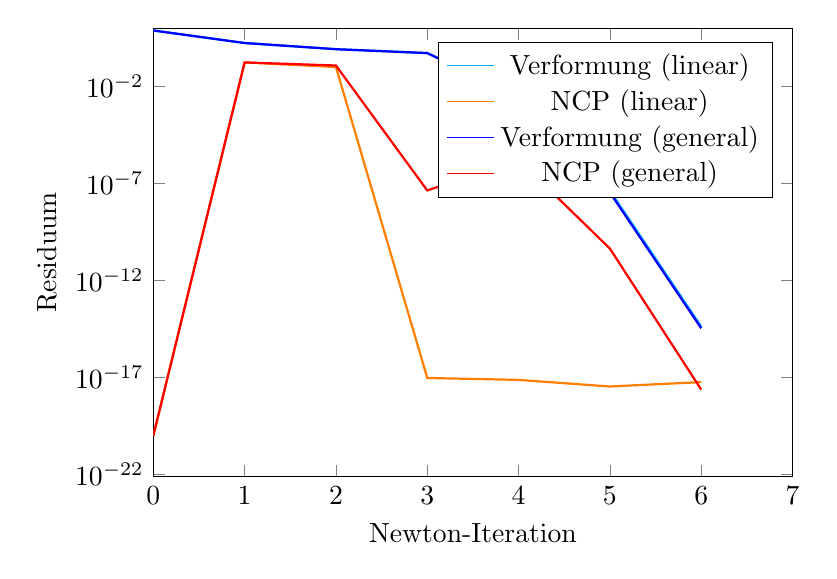
\begin{tikzpicture}[every plot/.append style={thick}] 
\begin{axis}[ 
label style={font=\normalsize}, 
xlabel={Newton-Iteration}, 
ylabel={Residuum}, 
xmin=0, xmax=7, 
ymode=log, 
ymin=0, ymax=10, 
width=0.8\textwidth, 
height=0.6\textwidth, 
legend pos=north east, 
legend style={cells={align=left}}, 
grid style=dashed, 
] 
\addplot[ 
color=cyan, 
] 
coordinates { 
(0, 7.64e+00)(1, 1.73e+00)(2, 8.32e-01)(3, 5.23e-01)(4, 2.96e-03)(5, 4.21e-08)(6, 4.19e-15)}; 
\addlegendentry{Verformung (linear)} 
\addplot[ 
color=orange, 
] 
coordinates { 
(0, 1.00e-20)(1, 1.73e-01)(2, 1.00e-01)(3, 9.54e-18)(4, 7.59e-18)(5, 3.47e-18)(6, 5.85e-18)}; 
\addlegendentry{NCP (linear)} 
\addplot[ 
color=blue, 
] 
coordinates { 
(0, 7.64e+00)(1, 1.73e+00)(2, 8.32e-01)(3, 5.25e-01)(4, 2.92e-03)(5, 3.42e-08)(6, 3.45e-15)}; 
\addlegendentry{Verformung (general)} 
\addplot[ 
color=red, 
] 
coordinates { 
(0, 1.00e-20)(1, 1.73e-01)(2, 1.20e-01)(3, 4.36e-08)(4, 1.68e-06)(5, 4.42e-11)(6, 2.39e-18)}; 
\addlegendentry{NCP (general)} 
\end{axis} 
\end{tikzpicture} 
\caption{Residuen des Stoffgesetzes 'Neo Hooke' mit Hinderniss 'Parabel' und 18 Freiheitsgraden für die Verschiebung.} 
\label{fiq:NeoHooke_Parabel_level0} 
\end{figure} 
